%% Measurement in Physical Education and Exercise Science — supplementary material, uploaded as a separate
%% file (published online via Figshare). Tables and figures are numbered S1, S2, ... in the order of their
%% first citation in main.tex, which refers to them through xr-hyper (prefix S-); this file refers to
%% main-text tables with prefix M-. The table bodies (t4, t5, s1 ... s8) are generated by
%% 08_r1_figurer_tabeller.py and 09_r1_supptex.py; their file names follow the generators, not the printed
%% numbers. The Supplementary Methods hold text moved from the main text for the MPEES page limit.

\documentclass[12pt,a4paper]{article}

\usepackage[utf8]{inputenc}
\usepackage[T1]{fontenc}
\usepackage{times}
\usepackage[margin=2.5cm]{geometry}
\usepackage{setspace}
\onehalfspacing

\usepackage{graphicx}
\graphicspath{{../figures/}}
\usepackage{float}
\usepackage{amsmath,amssymb}
\usepackage{booktabs}
\usepackage{xr-hyper}
\usepackage[colorlinks=true,linkcolor=blue,citecolor=blue,urlcolor=blue]{hyperref}
\externaldocument[M-]{main}[main.pdf]

\renewcommand{\thetable}{S\arabic{table}}
\renewcommand{\theHtable}{S\arabic{table}}
\renewcommand{\thefigure}{S\arabic{figure}}
\renewcommand{\theHfigure}{S\arabic{figure}}

\begin{document}

{\noindent\Large\bfseries\raggedright\hyphenpenalty=10000 Supplementary material\par}

\medskip
{\noindent\large\raggedright\hyphenpenalty=10000 How much is the wind worth? Sprints and horizontal jumps from age 10 to senior level\par}

\medskip
\noindent Atle G.\ Guttormsen and Simen Guttormsen. Tables and figures are numbered in the order of their first citation in the main text.

\section*{Supplementary Methods}

\subsection*{Sample construction: duplicate records}

Before the filters described in the main text (Section 2.1), we removed duplicate records: 47\,962 board-jump rows that re-imports in 2026 had copied from an identical take-off-zone result (same athlete, date, mark and wind; almost all at ages 11--13, and listed in the source only under the zone event), 8\,907 such copies from multi-day meets, dated to the meet's first day while the zone result lies one to six days later, and 770 exact duplicates, mostly meets stored twice. Because the 2026 import filed take-off-zone jumps under the board events, the 1\,597 board-event jumps at ages 11--13 in 2026 were also excluded.

\subsection*{Short hurdles}

The hurdles extension covers the ten short-hurdle event codes with substantive wind data (60 m to 110 m hurdles; each code specifies the class's hurdle height, so a code identifies an age-class specification), with the filters and estimator of the main events; the hurdles extension contributed 33\,205 analyzed rows. It was added after the main estimations by a post-plan decision.

In the age-class system, hurdle events carry class-specific heights, so each event code identifies an age-class specification. Across the ten codes with wind data (Table~\ref{tab:hurdles}; Figure~\ref{fig:hurdles}), the 60 m hurdles matched the flat 60 m of the same sex and class: 0.055--0.067 s per m/s against 0.056--0.070, point estimates from 21\,\% below to 9\,\% above the flat references, with overlapping intervals. Over 100 and 110 m the hurdle estimates mostly exceeded the flat 100 m reference, from 4\,\% below to 48\,\% above; in the girls' 76.2 cm class (0.108 against 0.082) the hurdle interval lies entirely above the flat interval, and in the boys' 84 cm class (0.133 against 0.090) it lies above the flat point estimate but overlaps the flat interval. Per second of race time the pooled hurdle codes (0.0048--0.0069 s per m/s) span the straight-sprint rates (Table~\ref{tab:sperdur}), so the hurdles' longer race times account for much of the difference, though not all of it in those two youth classes. Within the 100 m hurdles the youth codes also exceeded the senior code (0.108 s per m/s for girls' 76.2 cm at 16--17 and 0.133 for boys' 84 cm at 14--15, against 0.069 for the senior women's 84 cm event), although these comparisons cross sexes and hurdle heights.

\subsection*{Sample size: sensitivity analysis}

Because the sample is the eligible population (main text, Section 2.3), we report an a posteriori sensitivity analysis for the primary outcome, the wind slope in raw units (s or cm per m/s): the minimum detectable effect (MDE) of a two-sided Wald test of the meet-clustered slope at $\alpha$~=~0.05 with power 0.80, MDE~=~(1.96~+~0.84)~$\times$~SE, computed in Python from the estimated standard errors. The smallest effect size of interest is the slope at which a legal +2.0 m/s tailwind moves a mark by one recording unit: 0.005 s per m/s in the sprints, which are timed to 0.01 s, and 0.5 cm per m/s in the jumps, measured to 1 cm. At event level the MDE was 0.003 and 0.004 s per m/s in the 60 and 100 m and 0.4 and 0.3 cm in the long jump and its zone variant, all below that threshold, against 0.013 s in the 200 m, 0.018 and 0.053 s in the small 80 and 150 m events, and 0.9 and 1.4 cm in the two triple jumps. In the sex $\times$ age-band sprint models (main text, Table~\ref{M-tab:age}) it ranged from 0.004 to 0.086 s per m/s (median 0.014), largest for the 200 m at 10--11, one of the thin samples marked in Table~\ref{M-tab:window}. To protect precision, estimates are reported only where at least 300 results in 100 athlete-seasons contribute, and standard errors are clustered on meet, which gives wider intervals than the athlete clustering of the analysis plan. No participants were recruited, so no adjustment for attrition applies.

\subsection*{Departures from the analysis plan}

Besides the post-plan checks and extensions named in the main text, the analysis departed from the plan as follows. H5 is valued from the 0 to +2 m/s slope against a robust scale and for the sprints only (the plan named the +2.0 m/s advantage against the classical within-cell standard deviation, for all events); ability is the wind-adjusted rather than the raw season mean; the planned formal test of the age gradient (H2) was not run, and the age bands are reported with their intervals instead; the linear model uses readings within $\pm$8 rather than $\pm$5 m/s; and the drag-only benchmark, the per-second scaling, meet fixed effects by age band, the age-graded points, the 2025 lists, the sex- and age-specific asymmetry comparison (Table~\ref{tab:sasym}) and the external-sample comparison (Table~\ref{tab:selite}) were added after the plan.

\clearpage
\section*{Supplementary tables}

\begin{table}[H]
\centering
\caption{Robustness: gain per +1 m/s under alternative specifications (point estimates; s for sprints, cm for jumps).}
\label{tab:srobust}
\footnotesize
\resizebox{\textwidth}{!}{\begin{tabular}{lccccccc}
\toprule
Event & Primary & Cells $\geq$3 & No exact 0.0 & Excl. $\pm$0.2 of +2.0 & 2011--19 & 2021--26 & Meet FE \\
\midrule
60 m & 0.0591 & 0.0590 & 0.0591 & 0.0587 & 0.0600 & 0.0573 & 0.0513 \\
80 m & 0.0746 & 0.0711 & 0.0761 & 0.0743 & 0.0740 & 0.0779 & 0.0768 \\
100 m & 0.0823 & 0.0816 & 0.0823 & 0.0828 & 0.0843 & 0.0795 & 0.0659 \\
150 m & 0.0814 & --- & 0.0780 & 0.0865 & --- & --- & 0.0838 \\
200 m & 0.1215 & 0.1203 & 0.1215 & 0.1207 & 0.1258 & 0.1135 & 0.0713 \\
Long jump & 3.1498 & 3.1064 & 3.2449 & 3.2355 & 3.2396 & 3.0276 & 4.0094 \\
Long jump (zone) & 2.1133 & 2.0471 & 2.1538 & 2.1406 & 2.1337 & 2.1518 & 2.6624 \\
Triple jump & 4.1647 & 4.1451 & 4.2652 & 4.2381 & 3.8149 & 5.0653 & 6.2220 \\
Triple jump (zone) & 3.8821 & 3.3154 & 3.8589 & 3.7672 & 3.7075 & 4.8247 & 5.0930 \\
\bottomrule
\end{tabular}
}
\vspace{0.2em}
\parbox{0.97\textwidth}{\footnotesize Point estimates are identical under athlete and meet clustering; only intervals differ. The 150 m lacks the cells-$\geq$3 and period columns for want of data.}
\end{table}

\begin{table}[H]
\centering
\caption{Asymmetry: separate tail- and headwind slopes, observed head/tail ratio, and the ratio drag-only physics predicts for the same estimator (95\,\% CIs clustered on meet).}
\label{tab:asym}
\footnotesize
\resizebox{\textwidth}{!}{\begin{tabular}{llccccc}
\toprule
Event & Unit & Tailwind gain per +1 m/s & Headwind loss per $-$1 m/s & Ratio & $v^2$ benchmark & p equal slopes \\
\midrule
60 m & s & 0.047 (0.045--0.050) & 0.072 (0.069--0.075) & 1.51 & 1.18 & $<$0.001 \\
80 m & s & 0.072 (0.054--0.090) & 0.078 (0.060--0.095) & 1.07 & 1.17 & 0.741 \\
100 m & s & 0.065 (0.061--0.068) & 0.107 (0.102--0.112) & 1.66 & 1.14 & $<$0.001 \\
150 m & s & 0.093 (0.048--0.137) & 0.067 ($-$0.004--0.138) & 0.72 & 1.14 & 0.623 \\
200 m & s & 0.078 (0.068--0.087) & 0.184 (0.170--0.197) & 2.37 & 1.15 & $<$0.001 \\
Long jump & cm & 2.88 (2.63--3.14) & 2.88 (2.21--3.56) & 1.00 & --- & 0.999 \\
Long jump (zone) & cm & 2.48 (2.23--2.73) & 1.41 (1.02--1.80) & 0.57 & --- & $<$0.001 \\
Triple jump & cm & 4.55 (3.91--5.19) & 2.74 (1.28--4.21) & 0.60 & --- & 0.048 \\
Triple jump (zone) & cm & 4.69 (3.65--5.74) & 1.90 (0.16--3.64) & 0.40 & --- & 0.013 \\
\bottomrule
\end{tabular}
}
\vspace{0.2em}
\parbox{0.97\textwidth}{\footnotesize Drag-only ratio: time changes proportional to the change in squared airspeed at the athlete's mean speed, scaled to the observed linear slope, imposed on the observed winds and estimated with the same piecewise model. The simpler ratio $(2v+1)/(2v-1)$ for a wind of exactly $\pm$1 m/s is 1.14--1.18. No benchmark is given for the jumps, where wind acts on run-up and flight differently.}
\end{table}

\begin{table}[H]
\centering
\caption{The elite end with the same estimator: wind effects in US collegiate results (TFRRS) and in the career results of championship finalists (Tilastopaja), with the registry's all-age and senior rows as reference (within athlete $\times$ season; 95\,\% CIs and SEs clustered on meet).}
\label{tab:selite}
\scriptsize
\resizebox{\textwidth}{!}{\begin{tabular}{lrccccccccc}
\toprule
Sample & n & Mean mark & Per m/s, linear (95\,\% CI) & Per s & Tailwind & Headwind & Head/tail (drag) & 0 to +2 & Above +2 (SE) & Meet FE \\
\midrule
\multicolumn{11}{l}{\textit{100 m, men}} \\
Registry, all ages & 34\,165 & 12.40 & 0.080 (0.077--0.083) & 0.0064 & 0.066 & 0.101 & 1.54 (1.67) & 0.073 & 0.049 (0.005) & 0.064 \\
Registry, 20--34 & 8\,909 & 11.42 & 0.071 (0.066--0.075) & 0.0062 & 0.064 & 0.082 & 1.27 (1.58) & 0.073 & 0.047 (0.007) & 0.060 \\
US collegiate (TFRRS) & 57\,534 & 10.89 & 0.054 (0.053--0.056) & 0.0050 & 0.047 & 0.077 & 1.62 (1.67) & 0.051 & 0.043 (0.002) & 0.045 \\
Championship finalists (Tilastopaja) & 8\,885 & 10.19 & 0.048 (0.045--0.051) & 0.0047 & 0.036 & 0.070 & 1.93 (1.45) & 0.038 & 0.033 (0.005) & 0.040 \\
\multicolumn{11}{l}{\textit{100 m, women}} \\
Registry, all ages & 30\,392 & 13.84 & 0.085 (0.082--0.089) & 0.0062 & 0.065 & 0.114 & 1.77 (1.73) & 0.067 & 0.059 (0.006) & 0.071 \\
Registry, 20--34 & 4\,543 & 12.63 & 0.072 (0.067--0.078) & 0.0057 & 0.057 & 0.098 & 1.71 (1.58) & 0.055 & 0.063 (0.008) & 0.062 \\
US collegiate (TFRRS) & 63\,234 & 12.22 & 0.058 (0.056--0.060) & 0.0047 & 0.050 & 0.081 & 1.61 (1.76) & 0.059 & 0.041 (0.002) & 0.047 \\
Championship finalists (Tilastopaja) & 8\,047 & 11.25 & 0.059 (0.055--0.063) & 0.0052 & 0.044 & 0.083 & 1.86 (1.49) & 0.047 & 0.039 (0.008) & 0.053 \\
\multicolumn{11}{l}{\textit{200 m, men}} \\
Registry, all ages & 29\,352 & 27.07 & 0.117 (0.108--0.127) & 0.0043 & 0.071 & 0.183 & 2.56 (1.82) & 0.081 & 0.053 (0.015) & 0.067 \\
Registry, 20--34 & 4\,931 & 23.08 & 0.085 (0.068--0.101) & 0.0037 & 0.048 & 0.151 & 3.15 (1.64) & 0.070 & 0.013 (0.027) & 0.053 \\
US collegiate (TFRRS) & 57\,111 & 22.05 & 0.066 (0.062--0.069) & 0.0030 & 0.052 & 0.104 & 2.00 (1.64) & 0.057 & 0.045 (0.005) & 0.050 \\
Championship finalists (Tilastopaja) & 6\,265 & 20.54 & 0.065 (0.057--0.074) & 0.0032 & 0.030 & 0.114 & 3.74 (1.41) & 0.034 & 0.021 (0.016) & 0.068 \\
\multicolumn{11}{l}{\textit{200 m, women}} \\
Registry, all ages & 29\,894 & 29.86 & 0.125 (0.115--0.136) & 0.0042 & 0.083 & 0.185 & 2.22 (1.87) & 0.110 & 0.033 (0.015) & 0.077 \\
Registry, 20--34 & 2\,954 & 25.83 & 0.095 (0.075--0.115) & 0.0037 & 0.047 & 0.180 & 3.81 (1.76) & 0.071 & 0.011 (0.029) & 0.059 \\
US collegiate (TFRRS) & 71\,467 & 25.30 & 0.074 (0.070--0.078) & 0.0029 & 0.057 & 0.118 & 2.06 (1.81) & 0.072 & 0.040 (0.005) & 0.056 \\
Championship finalists (Tilastopaja) & 5\,804 & 22.93 & 0.078 (0.069--0.088) & 0.0034 & 0.055 & 0.110 & 2.00 (1.50) & 0.063 & 0.037 (0.022) & 0.079 \\
\multicolumn{11}{l}{\textit{100 m hurdles, women}} \\
US collegiate (TFRRS) & 61\,051 & 14.74 & 0.075 (0.072--0.079) & 0.0051 & 0.057 & 0.129 & 2.27 & 0.072 & 0.038 (0.005) & 0.062 \\
Championship finalists (Tilastopaja) & 7\,302 & 12.94 & 0.054 (0.049--0.059) & 0.0041 & 0.033 & 0.084 & 2.51 & 0.031 & 0.039 (0.010) & 0.045 \\
\multicolumn{11}{l}{\textit{110 m hurdles, men}} \\
US collegiate (TFRRS) & 45\,225 & 14.97 & 0.057 (0.054--0.060) & 0.0038 & 0.043 & 0.099 & 2.31 & 0.051 & 0.034 (0.004) & 0.043 \\
Championship finalists (Tilastopaja) & 6\,788 & 13.47 & 0.044 (0.039--0.050) & 0.0033 & 0.026 & 0.072 & 2.77 & 0.027 & 0.023 (0.009) & 0.046 \\
\multicolumn{11}{l}{\textit{Long jump, men}} \\
Registry, all ages & 15\,259 & 4.69 & 3.34 (2.90--3.78) & --- & 2.98 & 4.27 & 1.43 & 1.54 & 5.73 (0.60) & 4.77 \\
Registry, 20--34 & 1\,813 & 6.26 & 3.11 (1.69--4.52) & --- & 2.85 & 4.17 & 1.46 & 2.70 & 3.11 (1.71) & 8.56 \\
US collegiate (TFRRS) & 38\,335 & 6.77 & 3.74 (3.46--4.02) & --- & 3.88 & 3.18 & 0.82 & 4.97 & 2.58 (0.31) & 3.35 \\
Championship finalists (Tilastopaja) & 6\,279 & 7.95 & 4.53 (3.95--5.11) & --- & 4.08 & 6.42 & 1.57 & 4.89 & 2.40 (0.94) & 4.13 \\
\multicolumn{11}{l}{\textit{Long jump, women}} \\
Registry, all ages & 20\,515 & 4.17 & 3.04 (2.70--3.38) & --- & 2.88 & 3.40 & 1.18 & 2.51 & 3.58 (0.43) & 4.18 \\
Registry, 20--34 & 1\,536 & 5.43 & 4.15 (3.03--5.27) & --- & 3.99 & 4.88 & 1.22 & 4.38 & 3.42 (1.26) & 7.20 \\
US collegiate (TFRRS) & 50\,068 & 5.44 & 2.73 (2.52--2.94) & --- & 2.86 & 2.25 & 0.79 & 3.81 & 1.65 (0.23) & 2.37 \\
Championship finalists (Tilastopaja) & 6\,290 & 6.58 & 3.71 (3.27--4.16) & --- & 3.41 & 4.96 & 1.46 & 4.62 & 1.04 (0.58) & 2.84 \\
\multicolumn{11}{l}{\textit{Triple jump, men}} \\
Registry, all ages & 4\,237 & 11.15 & 4.21 (3.14--5.28) & --- & 5.18 & 1.27 & 0.25 & 3.39 & 8.50 (1.60) & 7.39 \\
Registry, 20--34 & 527 & 13.66 & 4.89 (2.55--7.23) & --- & 7.68 & $-$5.28 & -0.69 & 3.94 & 14.51 (4.48) & 10.77 \\
US collegiate (TFRRS) & 24\,224 & 14.25 & 4.57 (4.15--5.00) & --- & 4.27 & 5.76 & 1.35 & 5.54 & 2.68 (0.57) & 3.56 \\
Championship finalists (Tilastopaja) & 4\,801 & 16.85 & 6.55 (5.45--7.65) & --- & 5.74 & 9.50 & 1.65 & 5.83 & 5.54 (1.46) & 5.08 \\
\multicolumn{11}{l}{\textit{Triple jump, women}} \\
Registry, all ages & 7\,421 & 9.89 & 4.15 (3.41--4.90) & --- & 4.30 & 3.70 & 0.86 & 3.79 & 5.28 (1.14) & 6.02 \\
Registry, 20--34 & 1\,018 & 11.71 & 4.43 (3.14--5.72) & --- & 5.16 & 0.49 & 0.10 & 5.91 & 3.86 (1.80) & 6.30 \\
US collegiate (TFRRS) & 32\,378 & 11.68 & 3.94 (3.64--4.25) & --- & 3.78 & 4.60 & 1.22 & 4.90 & 2.34 (0.39) & 2.88 \\
Championship finalists (Tilastopaja) & 4\,467 & 14.21 & 5.89 (5.09--6.68) & --- & 5.86 & 6.00 & 1.02 & 6.88 & 3.66 (1.22) & 5.28 \\
\bottomrule
\end{tabular}
}
\vspace{0.2em}
\parbox{0.97\textwidth}{\footnotesize Sprints in seconds, jumps in centimeters, per m/s of wind, signed as gains with tailwind; n is the number of results in athlete-season-event cells with at least two wind-measured marks. Mean mark: all analyzed results (s for sprints, m for jumps), as in Table~\ref{tab:sperdur}. Per s: the linear gain divided by the mean time. The registry's 20--34 jump rows rest on thin samples. Tailwind and headwind: the separate branch slopes; head/tail: their ratio, with in parentheses the ratio drag-only physics predicts for the same winds and estimator at the athletes' own speeds (100 m and 200 m). 0 to +2 m/s and above +2 m/s: the tailwind slopes of the piecewise model used for H5. Meet FE: the linear slope with month dummies replaced by meet fixed effects. The registry's hurdle events are class-specific (Table~\ref{tab:hurdles}), so no registry row is given for the hurdles. The external estimates were stable across the registry's robustness variants (cells with at least three results, no exact-zero readings, athlete clustering; for the collegiate sample also without the 2016--2017 seasons, whose short careers the collection under-covers): the 100 and 200 m slopes moved by at most 3\,\%, and meet fixed effects attenuated the 100 m slopes by 10--20\,\% in all three samples. External samples: all outdoor results in the six events in the TFRRS profiles of NCAA Division I athletes (shared cleaned build, version 1.2), and the career results of athletes who reached a World Championships, Olympic or other major championship final 1983--2026 (Tilastopaja), after the registry's filters (electronic timing, wind within $\pm$8 m/s, event-specific plausibility bounds; combined-event sub-results excluded). Added after the analysis plan.}
\end{table}

\begin{table}[H]
\centering
\caption{Effect per second of race time: gain per +1 m/s divided by mean race duration, flat sprints and short hurdles.}
\label{tab:sperdur}
\footnotesize
\begin{tabular}{lccc}
\toprule
Event & Mean time (s) & Gain per +1 m/s (s) & Per second of race time \\
\midrule
60 m & 9.67 & 0.059 & 0.00610 \\
80 m & 12.58 & 0.075 & 0.00594 \\
100 m & 13.08 & 0.082 & 0.00629 \\
150 m & 20.22 & 0.081 & 0.00403 \\
200 m & 28.47 & 0.121 & 0.00427 \\
60 m hurdles 68 cm & 13.16 & 0.063 & 0.00478 \\
60 m hurdles 76.2 cm & 11.82 & 0.062 & 0.00525 \\
80 m hurdles 76.2 cm & 13.36 & 0.072 & 0.00536 \\
80 m hurdles 84 cm & 14.09 & 0.078 & 0.00550 \\
100 m hurdles 76.2 cm & 15.61 & 0.108 & 0.00693 \\
100 m hurdles 84 cm & 14.93 & 0.078 & 0.00523 \\
100 m hurdles 91.4 cm & 15.67 & 0.084 & 0.00534 \\
110 m hurdles 91.4 cm & 15.90 & 0.103 & 0.00646 \\
110 m hurdles 100 cm & 15.74 & 0.096 & 0.00612 \\
110 m hurdles 106.7 cm & 15.48 & 0.085 & 0.00548 \\
\bottomrule
\end{tabular}

\vspace{0.2em}
\parbox{0.8\textwidth}{\footnotesize Straight flat sprints cluster at 0.0059--0.0063 per m/s per second of race time; the bend events (150/200 m) sit about a third lower; hurdle codes bracket the flat rates.}
\end{table}

\begin{table}[H]
\centering
\caption{Wind effect in the horizontal jumps by age band (gain per +1 m/s; values girls/women / boys/men; 95\,\% CIs clustered on meet).}
\label{tab:sjumps}
\scriptsize
\resizebox{\textwidth}{!}{\begin{tabular}{llcccccc}
\toprule
Event & Unit & 10--11 & 12--13 & 14--15 & 16--17 & 18--19 & 20--34 \\
\midrule
Long jump & cm & --- & 2.63 (1.94--3.32) / 3.46 (2.46--4.46) & 2.89 (2.42--3.35) / 3.36 (2.82--3.89) & 3.04 (2.48--3.60) / 3.71 (2.68--4.74) & 3.20 (2.40--3.99) / 2.94 (1.58--4.29) & 4.15 (3.03--5.27) / 3.11 (1.69--4.52) \\
Long jump & \% & --- & 0.67 (0.49--0.85) / 0.88 (0.62--1.15) & 0.70 (0.58--0.82) / 0.76 (0.62--0.90) & 0.62 (0.49--0.76) / 0.66 (0.44--0.89) & 0.64 (0.46--0.82) / 0.48 (0.23--0.73) & 0.76 (0.53--1.00) / 0.49 (0.23--0.75) \\
Long jump (zone) & cm & 1.83 (1.41--2.24) / 2.39 (1.88--2.90) & 1.86 (1.59--2.14) / 2.54 (2.17--2.91) & --- & --- & --- & --- \\
Long jump (zone) & \% & 0.55 (0.42--0.68) / 0.70 (0.54--0.85) & 0.49 (0.41--0.56) / 0.66 (0.56--0.75) & --- & --- & --- & --- \\
Triple jump & cm & --- & 2.36 (0.08--4.65) / 6.58 (3.63--9.53) & 4.18 (3.07--5.29) / 4.20 (2.49--5.91) & 4.13 (2.88--5.37) / 4.10 (2.09--6.11) & 3.52 (1.68--5.36) / 4.21 (1.67--6.76) & 4.43 (3.14--5.72) / 4.89 (2.55--7.23) \\
Triple jump & \% & --- & 0.25 ($-$0.01--0.52) / 0.67 (0.35--1.00) & 0.45 (0.33--0.57) / 0.41 (0.24--0.58) & 0.40 (0.28--0.52) / 0.32 (0.15--0.49) & 0.31 (0.13--0.49) / 0.32 (0.12--0.52) & 0.37 (0.26--0.48) / 0.34 (0.17--0.51) \\
\bottomrule
\end{tabular}
}
\vspace{0.2em}
\parbox{0.97\textwidth}{\footnotesize In each cell the first value is girls/women, the second boys/men. The zone events are contested only in the youngest classes. In centimeters the effect rises with age for girls and women as jump distances and flight times grow; in percent it shows no consistent age direction.}
\end{table}

\begin{table}[H]
\centering
\caption{Wind effect in short hurdles by class-specific event code (sex-specific rows; flat-sprint reference for the same sex and distance class in that sex's modal age band for the code; 95\,\% CIs clustered on meet).}
\label{tab:hurdles}
\footnotesize
\resizebox{\textwidth}{!}{\begin{tabular}{llcccc}
\toprule
Event (hurdle height) & Sex & Modal band & Gain per +1 m/s (95\,\% CI), s & Flat reference (95\,\% CI), s & n \\
\midrule
60 m hurdles 68 cm & Boys & 10--11 & 0.055 (0.037--0.073) & 0.070 (0.066--0.075) & 1\,215 \\
60 m hurdles 68 cm & Girls & 10--11 & 0.067 (0.051--0.082) & 0.064 (0.060--0.068) & 2\,562 \\
60 m hurdles 76.2 cm & Boys & 12--13 & 0.063 (0.050--0.075) & 0.063 (0.060--0.066) & 3\,457 \\
60 m hurdles 76.2 cm & Girls & 12--13 & 0.062 (0.052--0.071) & 0.056 (0.054--0.059) & 7\,293 \\
80 m hurdles 76.2 cm & Girls & 14--15 & 0.072 (0.054--0.089) & --- & 2\,529 \\
80 m hurdles 84 cm & Boys & 14--15 & 0.078 (0.055--0.100) & --- & 1\,474 \\
100 m hurdles 76.2 cm & Girls & 16--17 & 0.108 (0.091--0.125) & 0.082 (0.077--0.086) & 1\,055 \\
100 m hurdles 84 cm & Boys & 14--15 & 0.133 (0.097--0.168) & 0.090 (0.085--0.094) & 709 \\
100 m hurdles 84 cm & Women & 20--34 & 0.069 (0.043--0.095) & 0.072 (0.067--0.077) & 2\,882 \\
100 m hurdles 91.4 cm & Boys & 16--17 & 0.084 (0.057--0.111) & 0.079 (0.074--0.083) & 685 \\
110 m hurdles 91.4 cm & Boys & 16--17 & 0.103 (0.044--0.162) & 0.079 (0.074--0.083) & 583 \\
110 m hurdles 100 cm & Men & 18--19 & 0.096 (0.044--0.149) & 0.078 (0.073--0.083) & 657 \\
110 m hurdles 106.7 cm & Men & 20--34 & 0.085 (0.051--0.119) & 0.071 (0.067--0.075) & 623 \\
\bottomrule
\end{tabular}
}
\vspace{0.2em}
\parbox{0.95\textwidth}{\footnotesize The hurdles analysis was added after the main estimations by a post-plan decision and is documented as a post-plan extension. Flat references are the 60 m or 100 m estimate for the same sex in that sex's modal age band; the flat 80 m has too few results at 14--15 for a reference. Codes with fewer than 300 results for one sex have only the other sex's row.}
\end{table}

\begin{table}[H]
\centering
\caption{Quadratic specification: linear and quadratic wind terms (raw outcome units per m/s: seconds for sprints, meters for jumps, e.g. 0.0328 m = 3.28 cm; SEs clustered on meet).}
\label{tab:squad}
\footnotesize
\begin{tabular}{lccc}
\toprule
Event & Linear term (SE) & Quadratic term (SE) & n \\
\midrule
100 m & -0.0856 (0.0008) & 0.0057 (0.0003) & 64,756 \\
150 m & -0.0794 (0.0171) & -0.0052 (0.0086) & 334 \\
200 m & -0.1306 (0.0021) & 0.0141 (0.0007) & 59,416 \\
60 m & -0.0595 (0.0006) & 0.0037 (0.0003) & 72,669 \\
80 m & -0.0752 (0.0054) & 0.0013 (0.0021) & 1,410 \\
Long jump & 0.0286 (0.0013) & 0.0001 (0.0004) & 51,870 \\
Long jump (zone) & 0.0194 (0.0009) & 0.0015 (0.0003) & 44,336 \\
Triple jump & 0.0372 (0.0032) & 0.0020 (0.0011) & 15,071 \\
Triple jump (zone) & 0.0342 (0.0051) & 0.0030 (0.0017) & 5,426 \\
\bottomrule
\end{tabular}
\vspace{0.2em}
\parbox{0.9\textwidth}{\footnotesize Negative linear terms for sprints mean faster times with tailwind. Positive quadratic terms in the large sprints match the headwind-tailwind asymmetry of Table~\ref{tab:asym}.}
\end{table}

\begin{table}[H]
\centering
\caption{Headwind/tailwind asymmetry on the 100 m by sex and age band, against drag-only physics at the athletes' own speeds (slopes in seconds per m/s, signed as gains with tailwind; 95\,\% CIs clustered on meet).}
\label{tab:sasym}
\scriptsize
\resizebox{\textwidth}{!}{\begin{tabular}{llrccccc}
\toprule
Sex & Age band & n & Mean time (s) & Tailwind slope & Headwind slope & Head/tail ratio (95\,\% CI) & Drag-only ratio \\
\midrule
Girls/women & 12--13 & 2\,733 & 14.80 & 0.083 & 0.112 & 1.35 (0.82--1.88) & 1.81 \\
Girls/women & 14--15 & 9\,740 & 13.93 & 0.071 & 0.126 & 1.76 (1.48--2.04) & 1.73 \\
Girls/women & 16--17 & 9\,062 & 13.41 & 0.059 & 0.112 & 1.91 (1.59--2.22) & 1.68 \\
Girls/women & 18--19 & 4\,207 & 13.04 & 0.064 & 0.106 & 1.66 (1.31--2.01) & 1.66 \\
Girls/women & 20--34 & 4\,543 & 12.57 & 0.057 & 0.098 & 1.71 (1.39--2.03) & 1.58 \\
Girls/women & All ages & 30\,392 & 13.53 & 0.065 & 0.114 & 1.77 (1.58--1.96) & 1.73 \\
Girls/women & All ages, meet FE & 30\,392 & 13.53 & 0.058 & 0.092 & 1.59 (1.35--1.83) & 1.70 \\
Boys/men & 12--13 & 1\,755 & 14.42 & 0.071 & 0.141 & 1.97 (0.87--3.07) & 1.92 \\
Boys/men & 14--15 & 7\,499 & 12.79 & 0.072 & 0.113 & 1.56 (1.28--1.85) & 1.73 \\
Boys/men & 16--17 & 9\,879 & 12.01 & 0.062 & 0.102 & 1.65 (1.37--1.93) & 1.59 \\
Boys/men & 18--19 & 6\,030 & 11.61 & 0.067 & 0.093 & 1.39 (1.03--1.75) & 1.55 \\
Boys/men & 20--34 & 8\,909 & 11.36 & 0.064 & 0.082 & 1.27 (1.01--1.52) & 1.58 \\
Boys/men & All ages & 34\,165 & 12.08 & 0.066 & 0.101 & 1.54 (1.36--1.71) & 1.67 \\
Boys/men & All ages, meet FE & 34\,165 & 12.08 & 0.055 & 0.080 & 1.46 (1.18--1.74) & 1.63 \\
\bottomrule
\end{tabular}
}
\vspace{0.2em}
\parbox{0.97\textwidth}{\footnotesize Head/tail ratio: headwind slope over tailwind slope, CI by the delta method. Drag-only ratio: time changes proportional to the change in squared airspeed at each athlete-season's mean speed, imposed on the observed winds and estimated with the same model (with meet fixed effects in the meet-FE rows). Added after the analysis plan.}
\end{table}

\begin{table}[H]
\centering
\caption{Correction table: tailwind slope over 0 to +2 m/s, and separate tail- and headwind slopes, by event, sex and age band (sprints; jumps event-level, in cm), with 95\,\% CIs clustered on meet.}
\label{tab:scorrection}
\scriptsize
\resizebox{\textwidth}{!}{\begin{tabular}{lllcccc}
\toprule
Event & Sex & Age band & Tailwind 0 to +2 & Tailwind slope per +1 m/s (95\,\% CI) & Headwind slope per $-$1 m/s (95\,\% CI) & n \\
\midrule
60 m & Boys/men & 10--11 & 0.057 & 0.055 (0.046--0.064) & 0.088 (0.077--0.098) & 7\,635 \\
60 m & Boys/men & 12--13 & 0.066 & 0.056 (0.050--0.062) & 0.071 (0.064--0.078) & 15\,457 \\
60 m & Boys/men & 14--15 & 0.054 & 0.042 (0.036--0.049) & 0.062 (0.051--0.073) & 6\,955 \\
60 m & Boys/men & 16--17 & 0.046 & 0.019 (0.004--0.035) & 0.064 (0.049--0.080) & 570 \\
60 m & Girls/women & 10--11 & 0.055 & 0.044 (0.036--0.052) & 0.085 (0.076--0.094) & 9\,794 \\
60 m & Girls/women & 12--13 & 0.057 & 0.047 (0.042--0.051) & 0.067 (0.062--0.072) & 21\,886 \\
60 m & Girls/women & 14--15 & 0.046 & 0.038 (0.032--0.043) & 0.068 (0.062--0.075) & 9\,320 \\
60 m & Girls/women & 16--17 & 0.030 & 0.021 (0.007--0.034) & 0.091 (0.068--0.113) & 389 \\
100 m & Boys/men & 12--13 & 0.082 & 0.071 (0.041--0.102) & 0.141 (0.111--0.170) & 1\,755 \\
100 m & Boys/men & 14--15 & 0.073 & 0.072 (0.063--0.081) & 0.113 (0.102--0.123) & 7\,499 \\
100 m & Boys/men & 16--17 & 0.069 & 0.062 (0.054--0.070) & 0.102 (0.094--0.111) & 9\,879 \\
100 m & Boys/men & 18--19 & 0.079 & 0.067 (0.058--0.077) & 0.093 (0.080--0.107) & 6\,030 \\
100 m & Boys/men & 20--34 & 0.073 & 0.064 (0.058--0.071) & 0.082 (0.071--0.092) & 8\,909 \\
100 m & Girls/women & 12--13 & 0.073 & 0.083 (0.062--0.105) & 0.112 (0.091--0.134) & 2\,733 \\
100 m & Girls/women & 14--15 & 0.073 & 0.071 (0.063--0.079) & 0.126 (0.116--0.135) & 9\,740 \\
100 m & Girls/women & 16--17 & 0.066 & 0.059 (0.052--0.066) & 0.112 (0.102--0.122) & 9\,062 \\
100 m & Girls/women & 18--19 & 0.072 & 0.064 (0.057--0.072) & 0.106 (0.092--0.120) & 4\,207 \\
100 m & Girls/women & 20--34 & 0.055 & 0.057 (0.050--0.064) & 0.098 (0.087--0.109) & 4\,543 \\
200 m & Boys/men & 10--11 & 0.133 & 0.107 (0.023--0.191) & 0.194 (0.090--0.298) & 1\,301 \\
200 m & Boys/men & 12--13 & 0.081 & 0.076 (0.041--0.111) & 0.217 (0.174--0.259) & 5\,443 \\
200 m & Boys/men & 14--15 & 0.079 & 0.078 (0.059--0.096) & 0.188 (0.164--0.212) & 7\,147 \\
200 m & Boys/men & 16--17 & 0.094 & 0.074 (0.060--0.088) & 0.172 (0.146--0.198) & 6\,372 \\
200 m & Boys/men & 18--19 & 0.063 & 0.069 (0.053--0.084) & 0.149 (0.124--0.173) & 4\,158 \\
200 m & Boys/men & 20--34 & 0.070 & 0.048 (0.026--0.070) & 0.151 (0.125--0.178) & 4\,931 \\
200 m & Girls/women & 10--11 & 0.256 & 0.099 (0.025--0.173) & 0.086 ($-$0.012--0.185) & 1\,780 \\
200 m & Girls/women & 12--13 & 0.127 & 0.105 (0.080--0.130) & 0.181 (0.143--0.219) & 7\,710 \\
200 m & Girls/women & 14--15 & 0.100 & 0.094 (0.075--0.113) & 0.186 (0.162--0.211) & 8\,640 \\
200 m & Girls/women & 16--17 & 0.091 & 0.066 (0.049--0.082) & 0.208 (0.173--0.243) & 5\,854 \\
200 m & Girls/women & 18--19 & 0.081 & 0.065 (0.047--0.082) & 0.151 (0.120--0.183) & 2\,956 \\
200 m & Girls/women & 20--34 & 0.071 & 0.047 (0.025--0.070) & 0.180 (0.143--0.218) & 2\,954 \\
Long jump & Both & all & --- & 2.98 (2.65--3.32) cm & 3.54 (2.68--4.41) cm & 40\,060 \\
Long jump (zone) & Both & all & --- & 2.48 (2.19--2.77) cm & 1.41 (0.95--1.87) cm & 44\,336 \\
Triple jump & Both & all & --- & 4.59 (3.80--5.39) cm & 2.82 (0.88--4.75) cm & 13\,068 \\
Triple jump (zone) & Both & all & --- & 4.69 (3.40--5.98) cm & 1.90 ($-$0.25--4.04) cm & 5\,426 \\
\bottomrule
\end{tabular}
}
\vspace{0.2em}
\parbox{0.97\textwidth}{\footnotesize Worked example: a girls' 12--13 100 m run in +1.8 m/s is corrected by $1.8 \times 0.073 = 0.13$ s to still air, using the slope over 0 to +2 m/s. Sprint slopes are in seconds; the four jump rows are in centimeters, pooled across bands. The 60 m rows at 16--17 rest on thin outdoor samples.}
\end{table}

\begin{table}[H]
\centering
\caption{Meet fixed effects by age band: effect per m/s of wind with month dummies replaced by meet fixed effects (seconds, 95\,\% CI clustered on meet), sprints.}
\label{tab:smeetfe}
\scriptsize
\resizebox{\textwidth}{!}{\begin{tabular}{llcccccc}
\toprule
Event & Sex & 10--11 & 12--13 & 14--15 & 16--17 & 18--19 & 20--34 \\
\midrule
60 m & Boys/men & 0.055 (0.045--0.066) & 0.055 (0.049--0.061) & 0.047 (0.040--0.055) & 0.030 (0.011--0.048) & --- & --- \\
60 m & Girls/women & 0.056 (0.049--0.063) & 0.049 (0.043--0.054) & 0.047 (0.041--0.052) & 0.030 (0.012--0.048) & --- & --- \\
100 m & Boys/men & --- & 0.107 (0.072--0.143) & 0.071 (0.056--0.085) & 0.063 (0.050--0.075) & 0.060 (0.046--0.073) & 0.060 (0.051--0.069) \\
100 m & Girls/women & --- & 0.093 (0.077--0.109) & 0.077 (0.066--0.089) & 0.065 (0.057--0.072) & 0.069 (0.059--0.080) & 0.062 (0.054--0.070) \\
200 m & Boys/men & $-$0.000 ($-$0.147--0.146) & 0.091 (0.054--0.128) & 0.078 (0.054--0.102) & 0.063 (0.038--0.088) & 0.058 (0.026--0.090) & 0.053 (0.033--0.072) \\
200 m & Girls/women & 0.030 ($-$0.082--0.142) & 0.087 (0.060--0.113) & 0.080 (0.061--0.100) & 0.079 (0.057--0.100) & 0.071 (0.047--0.094) & 0.059 (0.006--0.111) \\
\bottomrule
\end{tabular}
}
\vspace{0.2em}
\parbox{0.97\textwidth}{\footnotesize Same reporting threshold as Table~\ref{M-tab:age}. The 200 m at 10--11 has too few results per meet for the meet-FE estimate to be informative.}
\end{table}
\clearpage
\section*{Supplementary figures}

\begin{figure}[H]
\centering
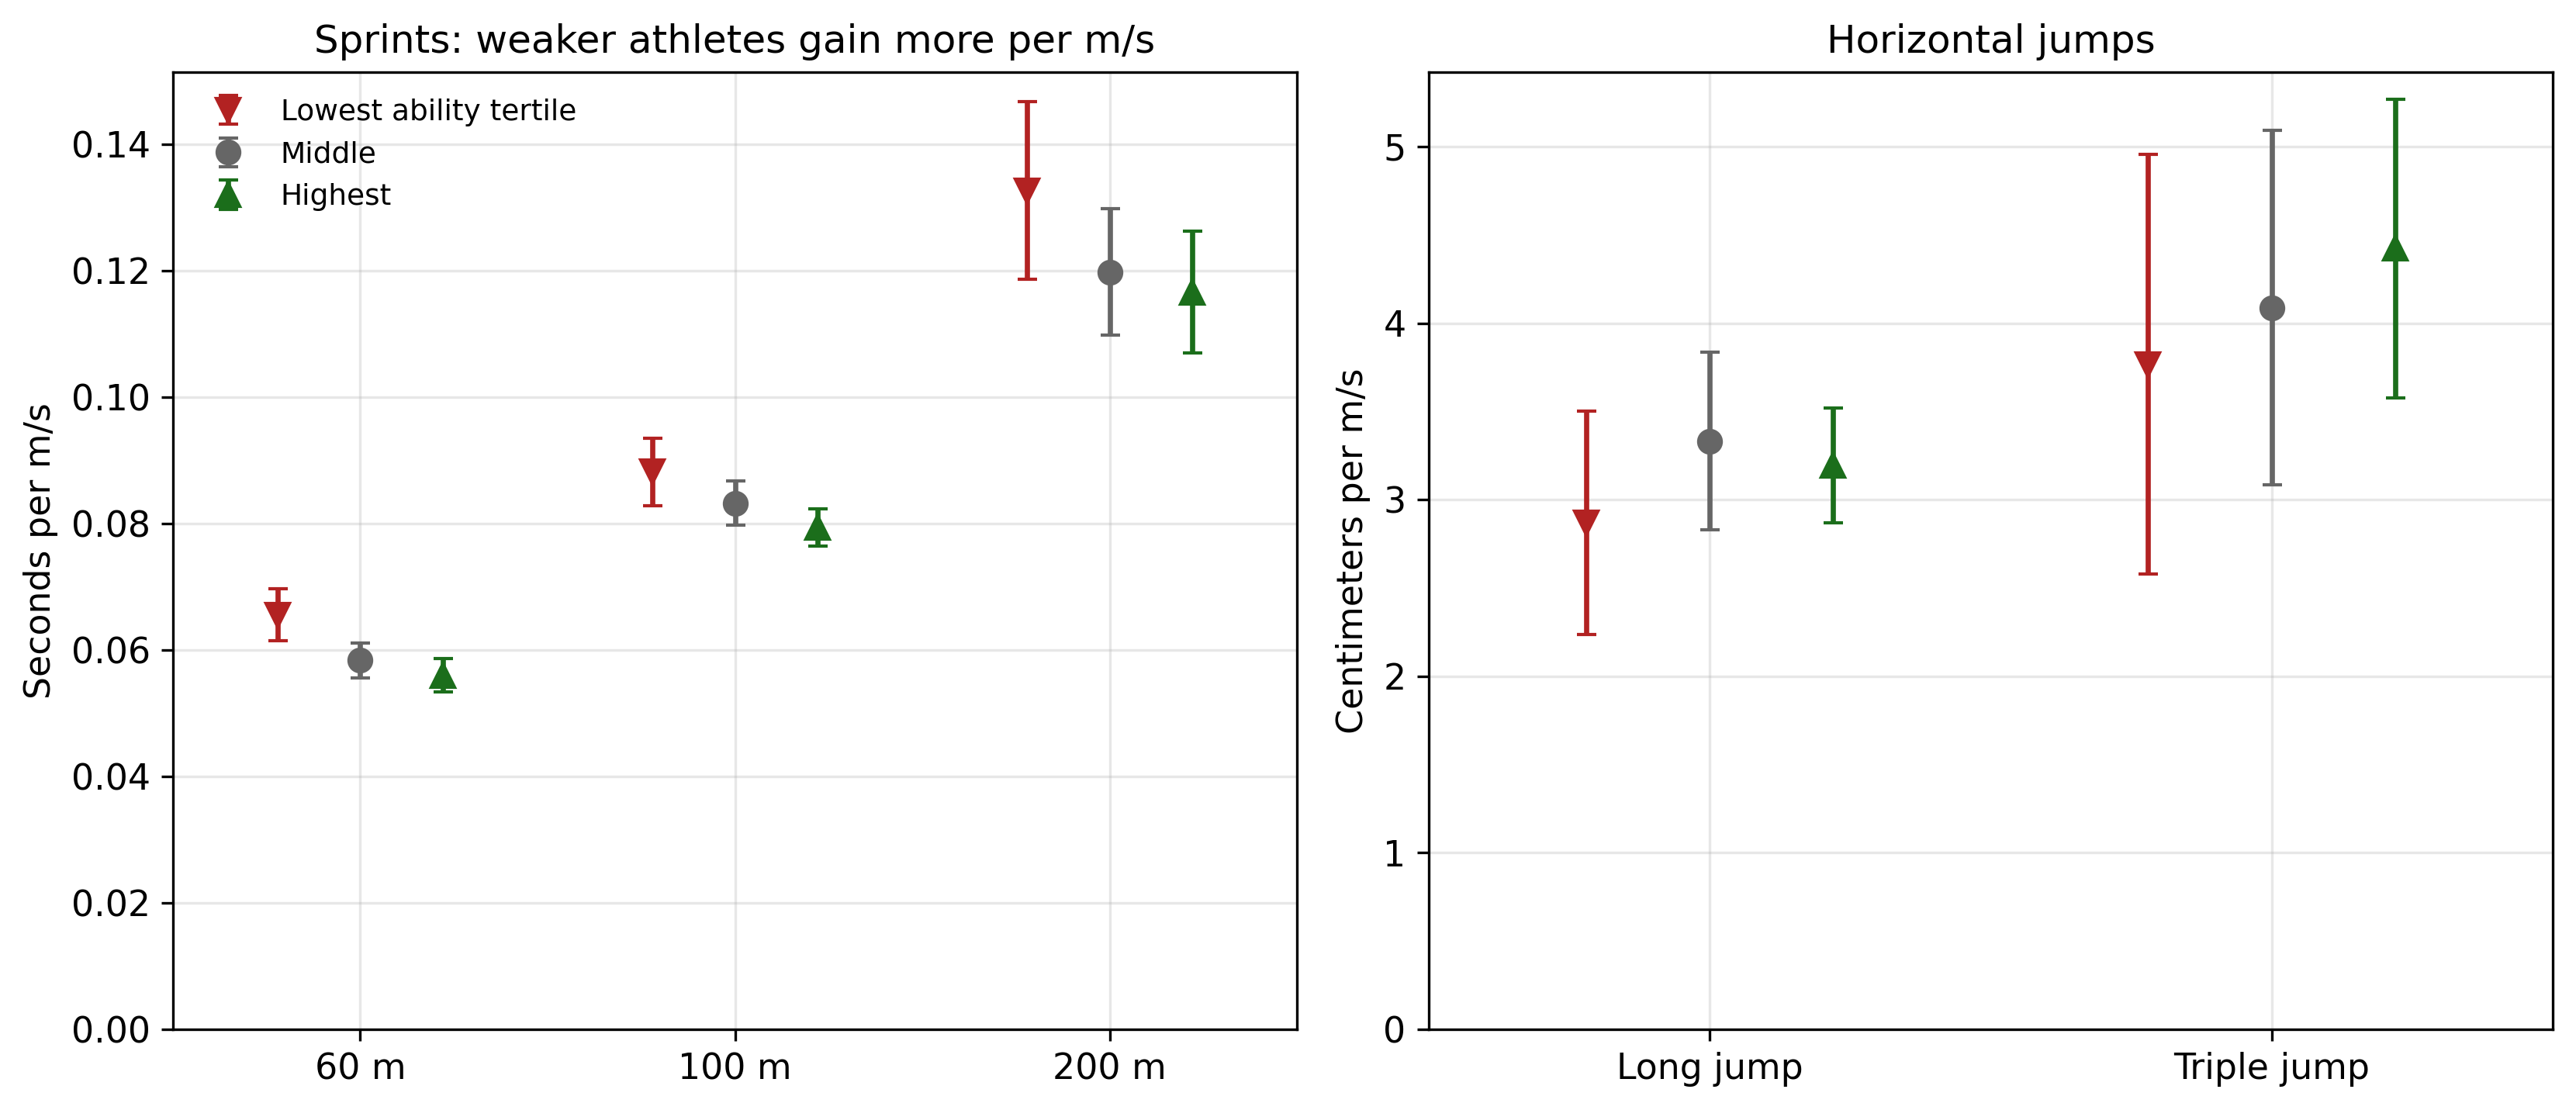
\includegraphics[width=\textwidth]{figS1_level.png}
\caption{Wind effect by ability tertile: athlete-seasons divided into equal thirds of the wind-adjusted season mean within event $\times$ sex $\times$ age band (points with 95\,\% CIs clustered on meet; lowest tertile downward triangles, middle circles, highest upward triangles).}
\label{fig:level}
\end{figure}

\begin{figure}[H]
\centering
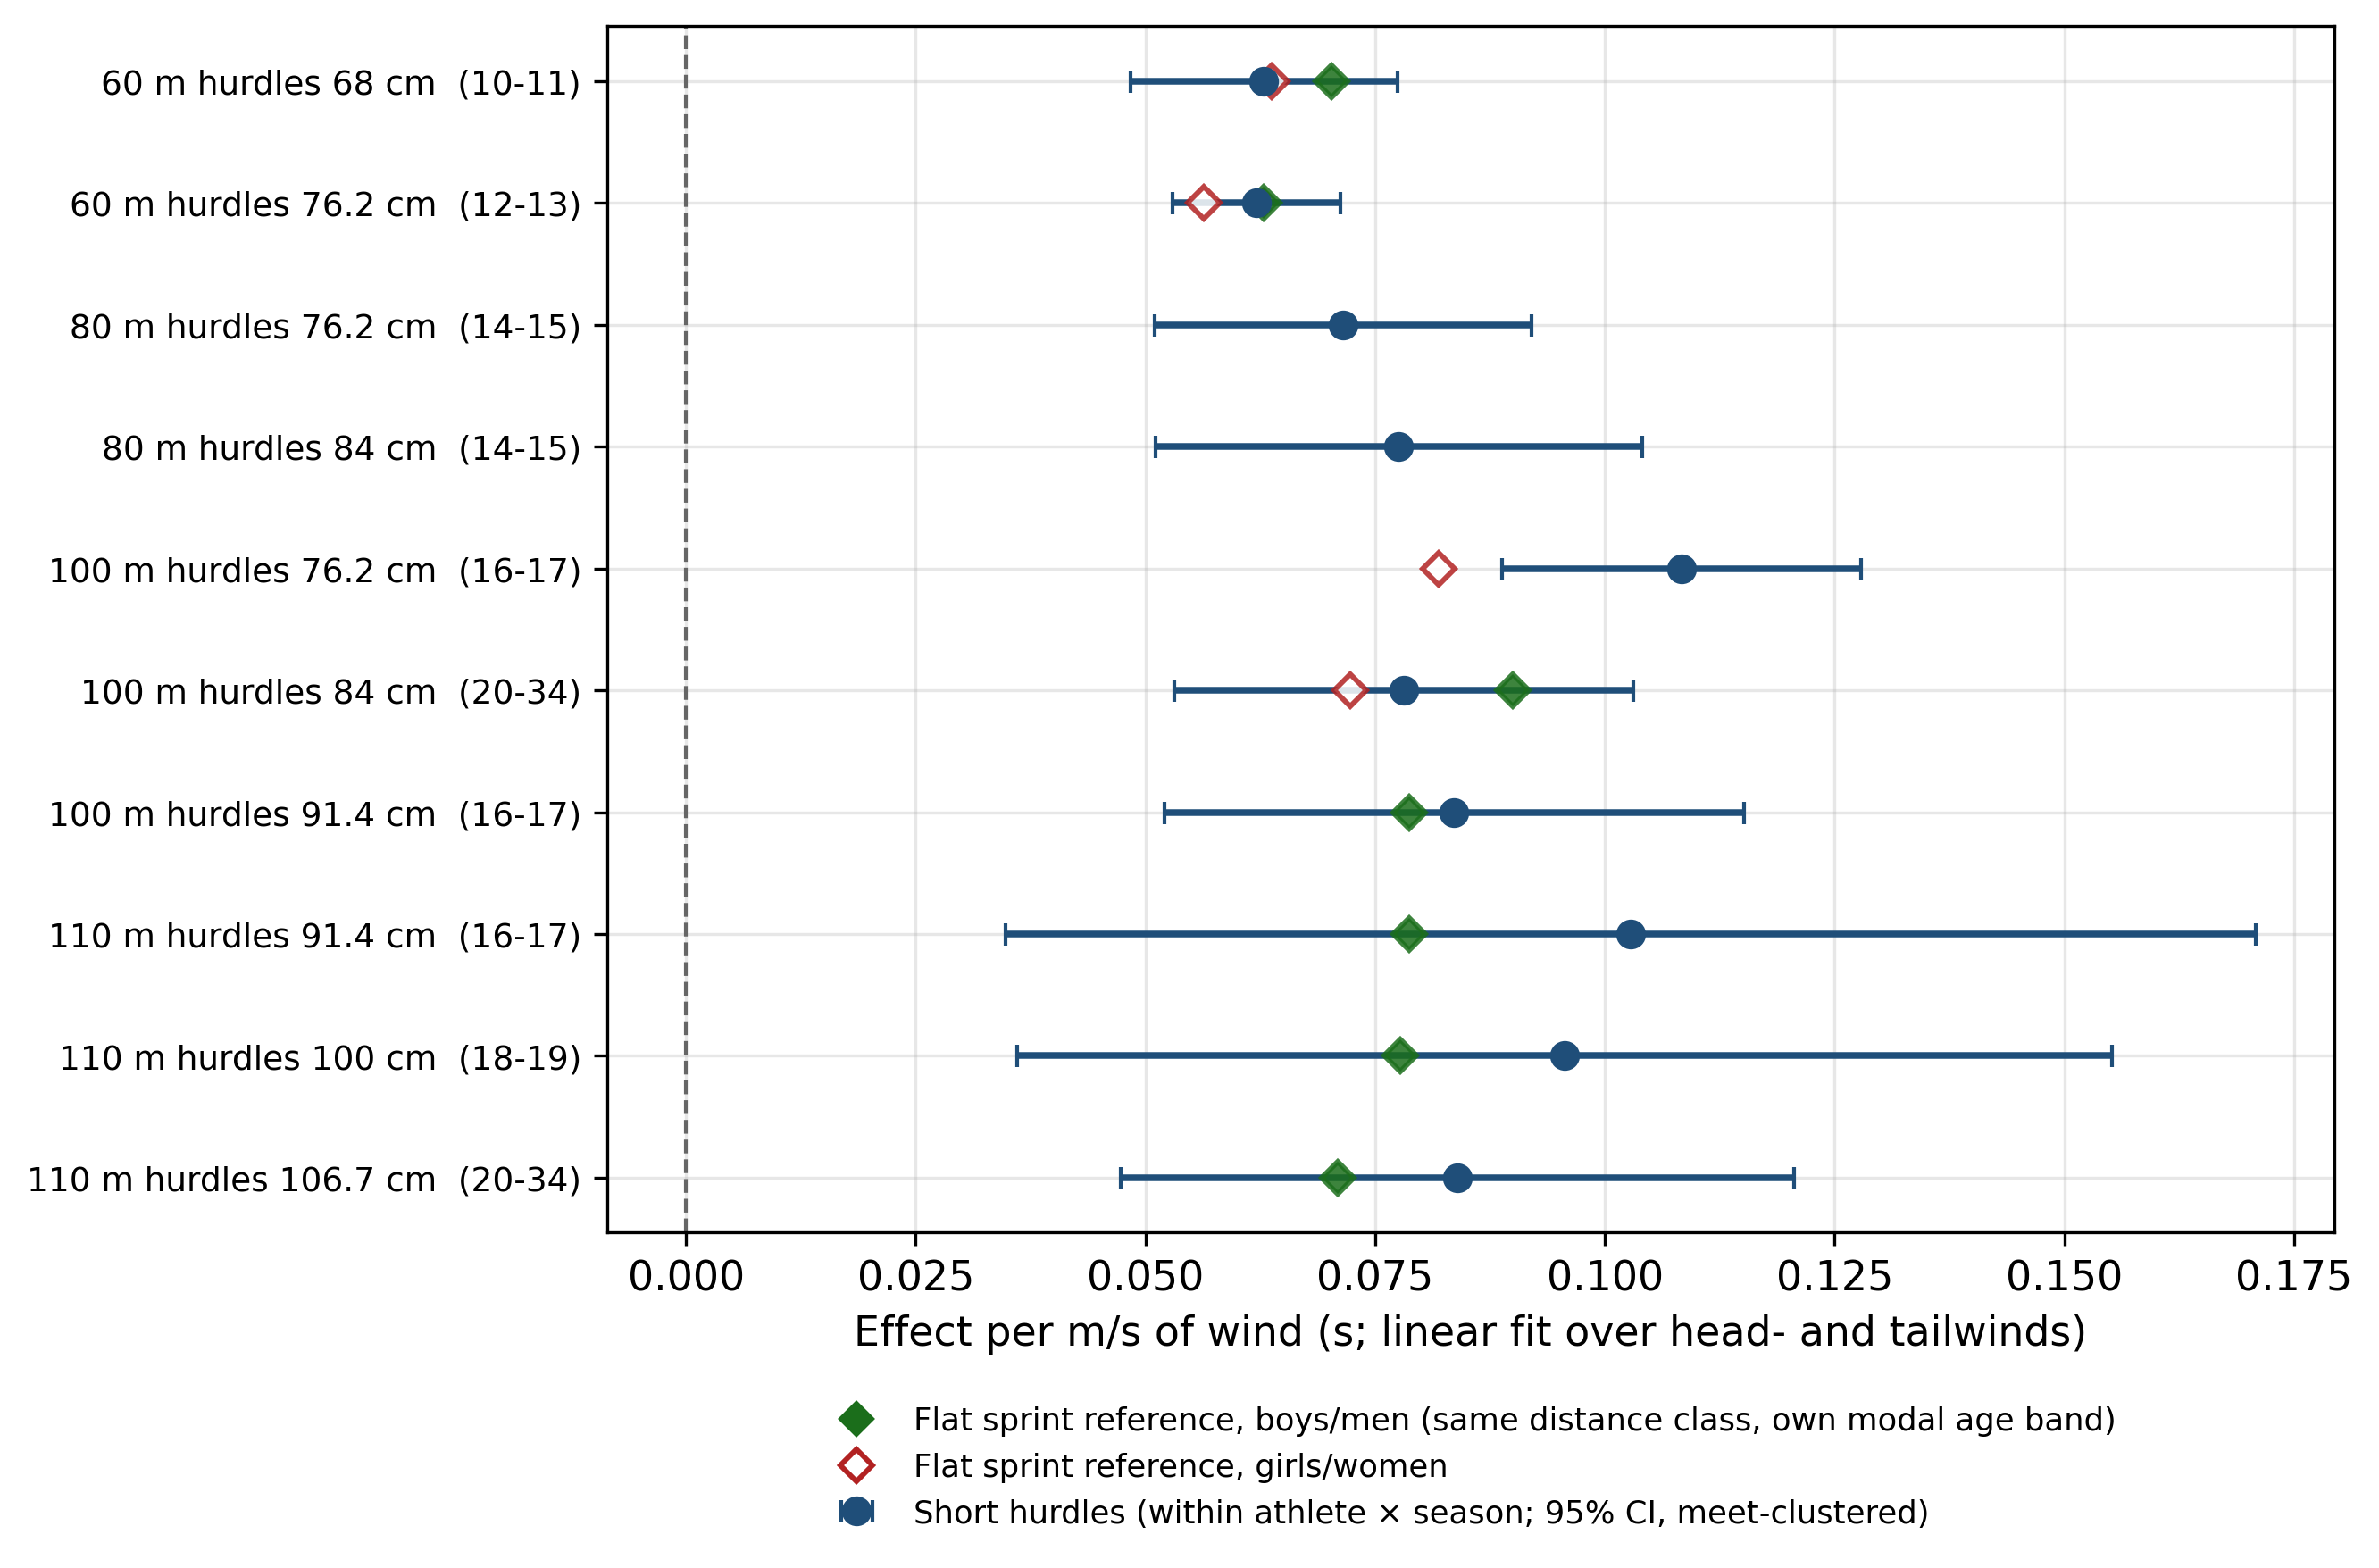
\includegraphics[width=0.95\textwidth]{figS2_hurdles.png}
\caption{Short hurdles: wind effect per class-specific code (pooled sexes; dots with 95\,\% CIs clustered on meet) against flat-sprint references for each sex (diamonds; boys/men filled, girls/women open).}
\label{fig:hurdles}
\end{figure}

\end{document}
